\section{An additional example of the phase shift dynamics}
\label{appendix:three-d-example}

In the~\Cref{fig:sa-example-run}, ~\Cref{fig:2-2-mce-example} and~\Cref{appendix:simple_goodharting_example}, we have explored an example of 2-state, 2-action MDP. The image space being 2-dimensional makes the visualisation of the run easy, but the disadvantage is that we do not get to see multiple state transitions. Here, we show an example of a 3-state, 2-action MDP, which does exhibit multiple changes in the direction of the optimisation angle.

We use an an MDP $\mathcal{M}_{3, 2}$ defined by the following transition matrix $\T$:

\begin{figure}[h]
    \centering
    \begin{subfigure}{.3\textwidth}
        \centering
        \begin{tabular}{|c|>{\color{orange}}c|>{\color{purple}}c|}
            \hline
            & $a_0$ & $a_1$ \\ [0.5ex] 
            \hline
            $S_0$ & 0.9 & 0.1 \\ [0.5ex]
            \hline
            $S_1$ & 0.1 & 0.9 \\ [0.5ex] 
            \hline
            $S_2$ & 0.0 & 0.0 \\ [0.5ex]
            \hline
        \end{tabular}
        \caption{$Starting\ from\ S_0$}
    \end{subfigure}%
    \begin{subfigure}{.3\textwidth}
        \centering
        \begin{tabular}{|c|>{\color{orange}}c|>{\color{purple}}c|}
            \hline
            & $a_0$ & $a_1$ \\ [0.5ex] 
            \hline
            $S_0$ & 0.1 & 0.9 \\ 
            \hline
            $S_1$ & 0.9 & 0.1 \\ 
            \hline
            $S_2$ & 0.0 & 0.0 \\ 
            \hline
        \end{tabular}
        \caption{$Starting\ from\ S_1$}
    \end{subfigure}
    \begin{subfigure}{.3\textwidth}
        \centering
        \begin{tabular}{|c|>{\color{orange}}c|>{\color{purple}}c|}
            \hline
            & $a_0$ & $a_1$ \\ [0.5ex] 
            \hline
            $S_0$ & 0.0 & 0.0 \\ 
            \hline
            $S_1$ & 0.0 & 0.0 \\ 
            \hline
            $S_2$ & 1.0 & 1.0 \\ 
            \hline
        \end{tabular}
        \caption{$Starting\ from\ S_2$}
    \end{subfigure}
\end{figure}

with $N=5$ different proxy functions interpolated linearly between $\R_0$ and $\R_1$. We use 30 optimisation strengths spaced equally between 0.01 and 0.99.

\begin{figure}[h]
\centering

\begin{subfigure}[t]{0.45\textwidth}
\centering
\begin{tabular}{|c|>{\color{orange}}c|>{\color{purple}}c|}
\hline
 & $a_0$ & $a_1$ \\
\hline
$S_0$ & 0.290 & 0.020 \\
\hline
$S_1$ & 0.191 & 0.202 \\
\hline
$S_2$ & 0.263 & 0.034 \\
\hline
\end{tabular}
\caption{Reward $\R_0$}
\end{subfigure}
\hfill
\begin{subfigure}[t]{0.45\textwidth}
\centering
\begin{tabular}{|c|>{\color{orange}}c|>{\color{purple}}c|}
\hline
 & $a_0$ & $a_1$ \\
\hline
$S_0$ & 0.263 & 0.195 \\
\hline
$S_1$ & 0.110 & 0.090 \\
\hline
$S_2$ & 0.161 & 0.181 \\
\hline
\end{tabular}
\caption{Reward $\R_1$}
\end{subfigure}

\caption{Reward Tables}
\end{figure}

The rest of the hyperparameters are set as in the~\Cref{appendix:simple_goodharting_example}, with the difference that we are now using exactly steepest ascent with early stopping, as described in~\Cref{alg:early-stopping-code}, instead of MCE approximation to it.

    
\begin{figure}[htbp]
    \centering
    \begin{subfigure}[tb]{0.45\textwidth}
        \centering
        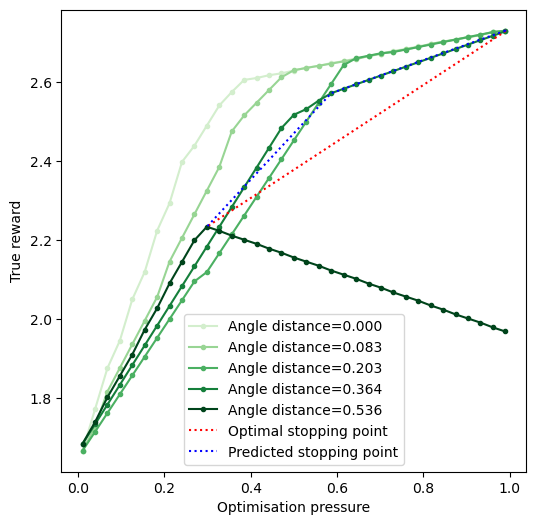
\includegraphics[width=0.8\textwidth]{example/example3d_run.png}
        \caption{Goodharting behavior for $\mathcal{M}_{3, 2}$ over five reward functions. Observe that the training method is concave, in accordance with~\Cref{prop:concave_proof}. Compare to the theoretical explanation in~\Cref{appendix:extra_explanation}, in particular to the figures showing piece-wise linear plots of obtained reward over increasing optimisation pressure.}
        \label{subfig:three-d-spatial}
    \end{subfigure}
    \hfill
    \begin{subfigure}[tb]{0.45\textwidth}
        \centering
        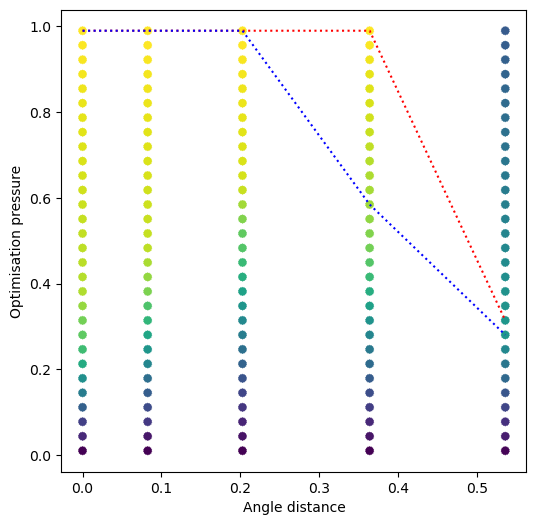
\includegraphics[width=0.8\textwidth]{example/example3d_lost.png}
        \caption{The same plot under a different spatial projection, which makes it easier to see how much the optimal stopping point differs from the pessimistic one recommended by the Early Stopping algorithm.\\ \\}
    \end{subfigure}
    \hfill
    \vspace{1cm}
    \begin{subfigure}[tb]{1\textwidth}
        \centering
        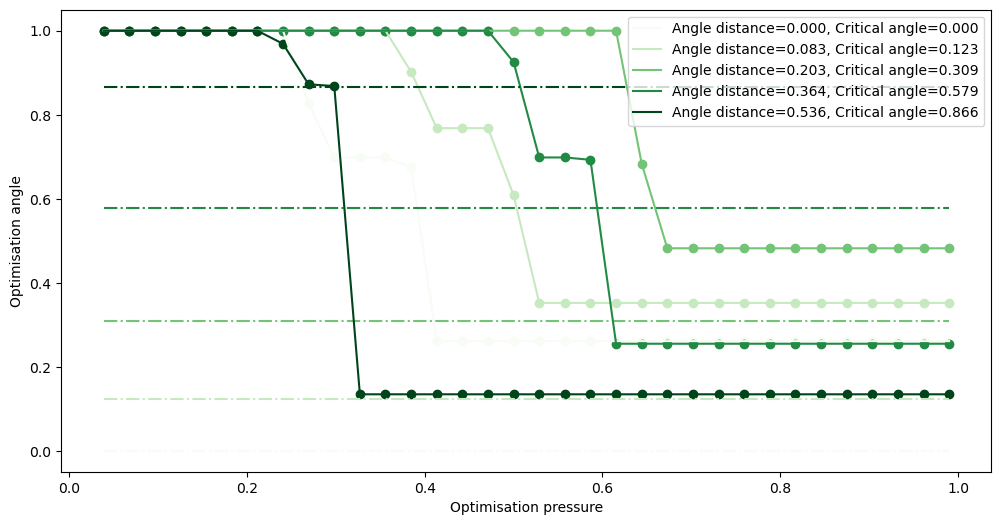
\includegraphics[width=0.8\textwidth]{example/example3d_angles.png}
        \caption{A visualisation of how the optimisation angle (cosine similarity) changes over increasing optimisation pressure for each proxy reward. This is the angle between the current direction of optimisation in $\Polytope$, i.e. $\left(\occmeas{\policy_{\alpha_{i+1}}}-\occmeas{\policy_{\alpha_i}}\right)$, and the proxy reward function projection $\QProj_\T\R_i$ (defined as $\CosDist{\VecProx}{\vec{d}}$ in the proof of~\Cref{thm:optimal_stopping}). Once the angle crosses the critical threshold, the algorithm stops. The critical threshold depends on the distance $\theta$ between the proxy and the true reward, and it is drawn in as a dotted line, with a color corresponding to the color of the proxy reward. Compare this plot to~\Cref{fig:goodhart-trends-five1} - we can see exact places where the phase transition happens, as the training run meets the boundary of the convex space. Also, compare to~\Cref{subfig:three-d-spatial}, where it can be seen how the algorithm stops (in blue) immediately after the training run crosses the corresponding critical angle value (in case fo the last two proxy rewards), or continues to the end (in case of the first two).}
    \end{subfigure}
    \caption{Summary plots for the Steepest Ascent training algorithm over five proxy reward functions.}
\end{figure}

\begin{figure}[htbp]
    \centering
    \begin{subfigure}[tb]{0.45\textwidth}
        \centering
        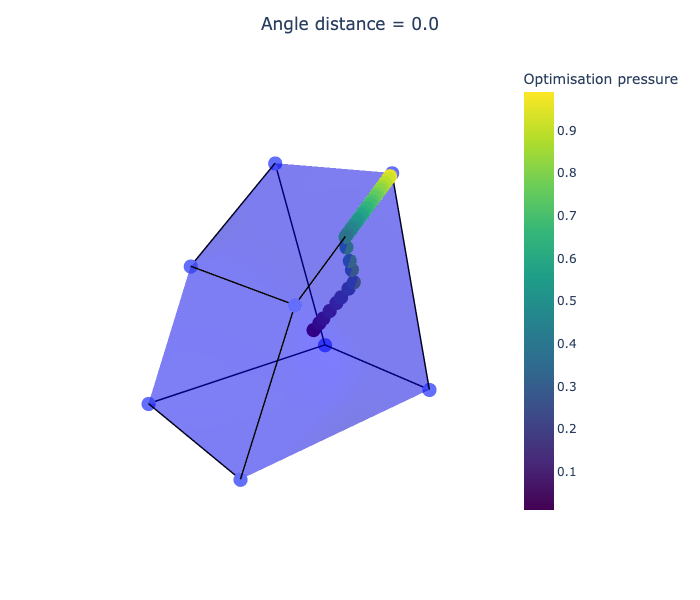
\includegraphics[width=1\textwidth]{example/example3d_0.png}
    \end{subfigure}
    \hfill
    \begin{subfigure}[tb]{0.45\textwidth}
        \centering
        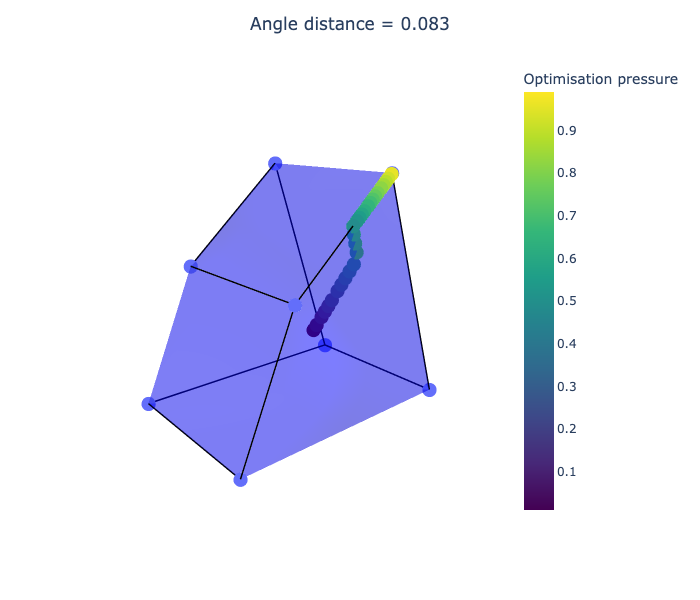
\includegraphics[width=1\textwidth]{example/example3d_1.png}
    \end{subfigure}
    \hfill
    \begin{subfigure}[tb]{0.45\textwidth}
        \centering
        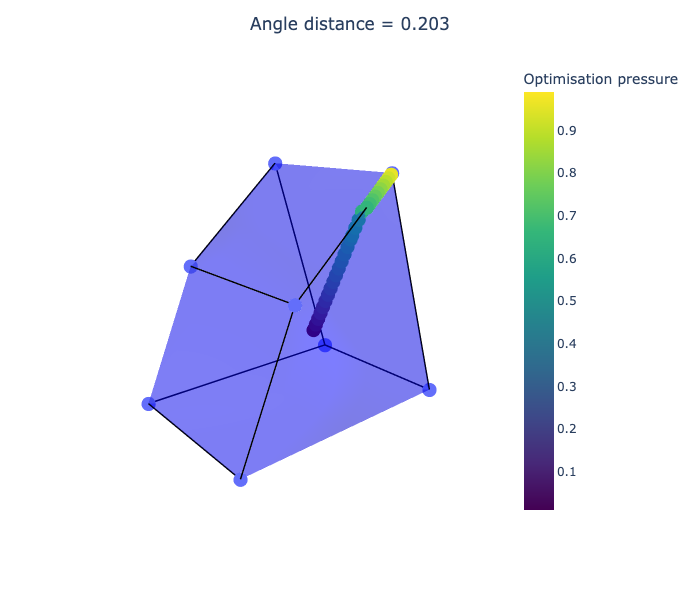
\includegraphics[width=1\textwidth]{example/example3d_2.png}
    \end{subfigure}
    \hfill
    \begin{subfigure}[tb]{0.45\textwidth}
        \centering
        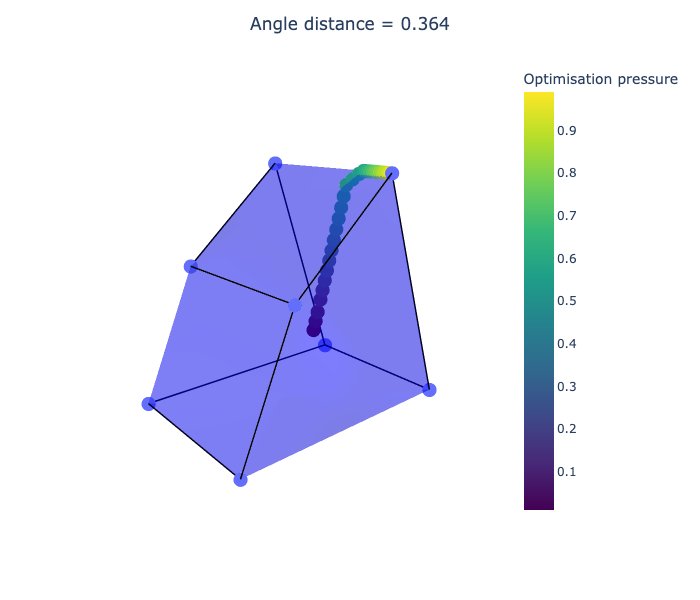
\includegraphics[width=1\textwidth]{example/example3d_3.png}
    \end{subfigure}
    \hfill
    \begin{subfigure}[tb]{0.45\textwidth}
        \centering
        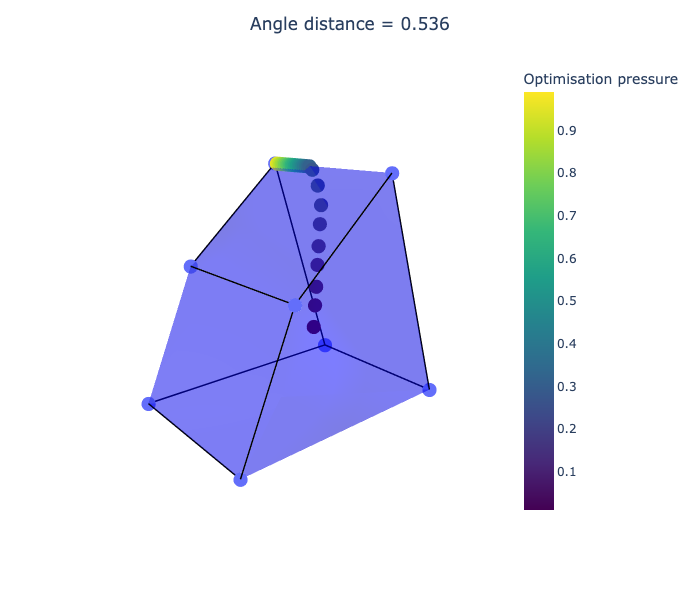
\includegraphics[width=1\textwidth]{example/example3d_4.png}
    \end{subfigure}
    \caption{Trajectories of optimisations for different proxy rewards. Note that the occupancy measure space is $|S|(|A| - 1) = 3$-dimensional in this example, and the convex hull is over $|A|^{|S|} = 8$ deterministic policies. We hide the true/proxy reward vector fields for presentation clarity.}
    \label{fig:goodhart-trends-five1}
\end{figure}

